\lstset{
  style              = Matlab-editor,
  basicstyle         = \mlttfamily,
  escapechar         = ",
  mlshowsectionrules = true,
}

\begin{filecontents*}{Bayes.m}
function [ result ] = Bayes( table )
    C = cvpartition(table2array(table(:,1)), 'HoldOut', 0.1);

    ens = fitcnb(table(C.training,:),'Type');
    % loss rate
    lossRate = loss(ens, table(C.test,:), 'Type');
    % confusion matrix
    prediction = predict(ens, table(C.test,:));
    confusionMatrix = confusionmat(table(C.test,:).Type, prediction);

    result = ClassificationResult(lossRate, confusionMatrix);
end
\end{filecontents*}

\begin{filecontents*}{KNN.m}
    ens = fitcknn(table(C.training,:),'Type');
\end{filecontents*}

\begin{filecontents*}{BoostedDecisionTree.m}
function [ result ] = boostedDecisionTree( table )
    C = cvpartition(table2array(table(:,1)), 'HoldOut', 0.1);

    ens = fitcensemble(table(C.training,:), 'Type', ...
        'Method', 'LogitBoost', 'NumLearningCycles', 500, 'LearnRate', 0.8,...
        'Learners', templateTree('MaxNumSplits',10, 'MinLeafSize', 8));
    % loss rate
    %[...]
\end{filecontents*}

\begin{filecontents*}{NeuralNetwork.m}
function [ result ] = neuronalNetwork( table )
    %transform feature table
    %[...]    
    %initialize the neural network
    net = patternnet([20, 20], 'trainlm');    
    [net,tr] = train(net,inputs,targets);    
    %evalute the neural network
    outputs = net(inputs);
    % loss rate
    %[...]
end
\end{filecontents*}

\section{Klassifikatoren} \label{Klassifikatoren}
Bei der Entwicklung der Klassifikation von Schüttgut wurde ein Ansatz verfolgt, der einen einfachen Austausch des Klassifikators erlaubt. In der Folge konnten mehrere verschiedene Klassifikatoren getestet und verglichen werden. Die Klassifikatoren wurden mit Hilfe der Matlab Toolboxen \textit{Statistics and Machine Learning Toolbox} \cite{MLToolbox} und \textit{Neural Network Toolbox} \cite{NNToolbox} erstellt. In Kapitel~\ref{NaiveBayes} wird ein Naive Bayes Klassifikator beschrieben und in Kapitel~\ref{KNN} ein k-Nearest-Neighbour Klassifikator. Für die beiden vielversprechendsten Klassifikatoren Boosted Decision Trees (vgl. Kapitel~\ref{BDT}) und Neuronal Networks (vgl. Kapitel ~\ref{NN}) wurden sowohl das Lernverfahren, als auch die Parameter der Klassifikatoren optimiert.

\subsection{Naive Bayes} \label{NaiveBayes}
Der von Marrakchi in seiner Arbeit \cite{MA} erstellte Naive Bayes Klassifikator konnte nicht ohne weiteres in unseren Arbeit integriert werden. Daher haben wir einen eigenen Bayes Klassifikator erstellt. Die Ergebnisse dieses Klassifikators stellen die Referenzwerte dar, mit denen wir unsere optimierten Klassifikatoren vergleichen.

Der Bayes Klassifikator bekommt die extrahierten Features (vgl. Kapitel~\ref{Features}) von zwei zu trennenden Schüttgutklassen als Eingabe. Von diesen Daten werden 10\% abgetrennt und zur Crossvalidierung verwendet (Listing~\ref{lst:Bayes.m}, Zeile 2). Die eigentliche Klassifikation der Partikel erfolgt in zwei Schritten. Im Trainingsschritt werden anhand der Trainingsdaten die Parameter der Wahrscheinlichkeitsverteilung geschätzt (Listing~\ref{lst:Bayes.m}, Zeile 4). Im Vorhersageschritt werden die Partikel der Testdaten anhand ihrer a posteriori Wahrscheinlichkeit einer Schüttgutklasse zugeordnet (Listing~\ref{lst:Bayes.m}, Zeile 8).
% https://de.mathworks.com/help/stats/naive-bayes-classification.html

\begin{minipage}{\textwidth}
\lstinputlisting[caption = {Bayes Klassifikator in Matlab},label={lst:Bayes.m}]{Bayes.m}
\end{minipage}



\subsection{k-Nearest-Neighbours} \label{KNN}
Der k-Nearest-Neighbour Klassifikator ist analog zum Bayes Klassifikator aufgebaut. Zunächst werden 10\% der Eingabedaten für die Crossvalidierung abgeschnitten, anschließend wird der Klassifikator in einem Trainingsschnitt trainiert. Da der Algorithmus dieses Klassifikators in der Statistics and Machine Learning Toolbox enthalten ist, muss hierzu lediglich die fitting function \cite{FittingFunctions} ausgetauscht werden (vgl. Listing~\ref{lst:KNN.m}).

\lstinputlisting[caption = {Auszug KNN Klassifikator in Matlab},label={lst:KNN.m}]{KNN.m}



\subsection{Boosted Decision Trees} \label{BDT}
Der letzte Klassifikator, der mit Hilfe der Machine Learning Toolbox entstanden ist, ist ein Boosted Decision Tree Klassifikator (vgl. Listing \ref{lst:BoostedDecisionTree.m}). Der Aufbau bezüglich der Partitionierung der Trainingsdaten (vgl. Listing \ref{lst:BoostedDecisionTree.m}, Zeile 2) und der Auswertung der Loss Funktion (vgl. Listing \ref{lst:BoostedDecisionTree.m}, Zeile 7) ist mit den in den Abschnitten \ref{NaiveBayes} und \ref{KNN} vorgestellten Klassifikatoren identisch.

Im Gegensatz zu diesen Klassifikatoren verwenden wir hier allerdings nicht nur einen Lernalgorithmus, sondern eine Methode des Ensemble Learning. Statt eines einzelnen Entscheidungsbaums, der zu einer hohen Fehlerrate neigt, benutzen wir ein Ensemble an Entscheidungsbäumen, die alle zur Klassifikation beitragen. Wir verwenden hier einen Ansatz, der unter dem Namen Boosting bekannt ist und erstmals von Freund und Schapire \cite{Freund1997} beschrieben wurde. Hierbei werden mehrere schwache Klassifikatoren kombiniert, um einen starken Klassifikator zu erhalten. Ein schwacher Klassifikator ist dabei ein Klassifikator, der zumindest leicht besser ist, als zufälliges Raten. Für dieses allgemeine Verfahren gibt es mehrere Implementierungen, von denen die beiden bekanntesten in der Machine Learning Toolbox enthalten sind:

\paragraph{AdaBoost} erhält als Eingabe ein Trainingsdatenset. Für dieses Set wird eine Verteilung D an Gewichten angelegt. Die Gewichte werden dabei mit dem gleichen Wert initialisiert. AdaBoost führt dann T mal den schwachen Klassifikator aus. Der Klassifikator findet dabei eine schwache Hypothese. Diese Hypothese wird nach der Anzahl richtig klassifizierten Beispiele gewichtet. Anschließend werden die Gewichte für die Verteilung D so angepasst, dass falsch klassifizierte Beispiele für den nächsten Durchlauf stärker gewichtet werden, damit diese vom schwachen Klassifikator mehr Aufmerksamkeit bekommen.

Am Ende entsteht der starke Klassifikator aus einem gewichteten Mehrheitsentscheid der schwachen Klassifikatoren \cite{Boosting03_Schapire}.
% Muss das genauer beschrieben werden? Pseudocode?


\paragraph{LogitBoost} Ist eine Abwandlung von AdaBoost bei der die Kostenfunktion, die AdaBoost zugrunde liegt, abgeändert wurde \cite{Friedman00specialinvited}.
% TODO: genauer

Boosting Ansätze sind im Allgemeinen nicht anfällig für overfitting. Selbst wenn keine Fehler mehr im Training auftreten, schaden weitere Durchläufe nicht, sondern verfeinern den Klassifikator weiter, da er für die richtig klassifizierten Daten eine höhere Sicherheit erhält \cite{ExplainingAdaBoost_Schapire}.

Bei den uns zur Verfügung stehenden Simulationsdaten der Partikel ist zwar kein Rauschen vorhanden, dennoch haben wir bei der Wahl eines geeigneten Boosting Verfahrens die Einflüsse in der realen Welt berücksichtigt. In empirischen Tests hat sich LogitBoost als resistenter gegenüber Rauschen herausgestellt \cite{McDonald2003}.

In unseren Tests hat sich ein Boosted Decision Tree mit der Methode LogitBoost und 500 Lernzyklen mit einer Lernrate von 0,8 als die gute Wahl erwiesen (vgl. Listing \ref{lst:BoostedDecisionTree.m}, Zeile 7 ff.). Die Anzahl der Lernzyklen beschreibt dabei, wie bereits erwähnt, die Häufigkeit der Ausführung des schwachen Klassifikators. Die Lernrate beeinflusst die Rate, mit der die Verlustfunktion minimiert wird. Je kleiner der Wert, desto mehr Zyklen müssen ausgeführt werden. Dadurch wird das Verfahren jedoch auch präziser.   
Außerdem darf sich der Entscheidungsbaum maximal 10 mal teilen und er muss mindestens 8 Blätter haben.
%TODO:Warum ist das so? (Benno)

\begin{minipage}{\textwidth}
\lstinputlisting[caption = {Boosted Decision Tree Klassifikator in Matlab},label={lst:BoostedDecisionTree.m}]{BoostedDecisionTree.m}
\end{minipage}

\subsection{Neural Network} \label{NN}
Mit der Neural Network Toolbox und der Funktion \textit{patternet} lässt sich in Matlab ein Neuronales Netz zur Klassifikation erstellen. Hierbei wird die Struktur des Netzes, also die Anzahl der Neuronen von jeder verborgenen Neuronenschicht, als Eigenvektor übergeben. Außerdem wird eine Trainingsfunktion und Performance-Funktion übergeben (vgl. Listing \ref{lst:NeuralNetwork.m}, Zeile 5).

Wie bei den anderen Klassifikatoren wird auch hier der Datensatz eingeteilt. Dies geschieht automatisch in der \textit{patternnet} Funktion. Die Auswahl an Testdaten, Validierungsdaten und Trainingsdaten erfolgt dabei zufällig. Die standardmäßige Unterteilung ist dabei wie folgt: 15\% Testdaten, 15\% Validierungsdaten und 70\% Trainingsdaten \cite{NNDivideData}.

Ein so entworfenes Neuronales Netz besteht aus einer Eingabeschicht, beliebig vielen verborgenen Neuronenschichten und einer Ausgabeschicht. Die Eingabe- und Ausgabeschicht ist durch unser Klassifikationsproblem vorgegeben. Die Anzahl der Neuronen in der Eingabeschicht ist dabei abhängig von der Dimension der gewählten Features. Die Ausgabeschicht hat zwei Neuronen, da wir zwei unterschiedliche Schüttgutklassen trennen wollen. Nach Hagan et altera haben die meist verwendeten Neuronalen Netze lediglich zwei oder drei Schichten
%(TODO Kapitel 2-12)
\cite{NNDesign}. Die Wahl der Anzahl der Neuronen in diesen Schichten ist nicht trivial und ist ein aktuelles Forschungsgebiet.

Das Ziel beim Entwurf eines Neuronalen Netzes ist es eine hohe Generalisierung zu erreichen. Das Netz soll insbesondere nicht overfitten. Beim Overfitting lernt das Netz die Daten einfach auswendig und versteht nicht die Unterschiede der Klassen. Um dies zu erreichen versucht man das allgemeinste Modell zu finden, welches das Klassifikationsproblem löst. Dieser Ansatz ist als Ockham's Razor bekannt.
%ToDo sollte noch mal mit Benno besprochen werden

Um Overfitting zu vermeiden, gibt es mehrere Möglichkeiten. Beim \textit{growing} wird die Anzahl der Neuronen in den verborgenen Schichten langsam erhöht, bis das Netz gut klassifiziert. Beim \textit{pruning} wird mit einem großen Netz begonnen und die Anzahl der Neuronen so lange verringert, bis das Netz schlechter wird. Die \textit{Regularization} ist eine Methode, um die Performance Funktion so zu verändern, dass eine höhere Komplexität des Netzes bestraft wird. 

Wir haben uns mit einem Verfahren beschäftigt, das in der Neural Network Toolbox bereits implementiert ist: Dem \textit{Early Stopping}. Die Idee hinter early stopping ist, dass immer mehr Gewichte im Netz angepasst werden, je länger das Training dauert. Folglich wird mit jeder weiteren Trainingsepoche die Komplexität des Netzes erhöht. Um dies zu verhindern, muss der Trainingsprozess früher gestoppt werden. Als Abbruchkriterium wird hierbei die Klassifizierung auf den Validierungsdaten verwendet. Sobald eine Verbesserung der Klassifikation nur noch auf den Trainingsdaten stattfindet, für die Validierungsdaten aber gleich bleibt oder sogar schlechter wird, bricht das Training ab.

In unseren Tests hat sich ein Neuronales Netz mit der Struktur wie in Abbildung \ref{fig:NNStructure} als besonders gut erwiesen. Das Netz besteht aus zwei versteckten Schichten mit jeweils 20 Neuronen.

\begin{figure}[!h] \label{NNStructure}
    \centering
    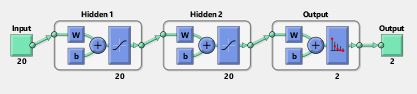
\includegraphics[width=1\textwidth]{pics/NN-Structure.JPG}
    \caption{Struktur des Neuronalen Netzes}
    \label{fig:NNStructure}
\end{figure}

Die verwendete Trainingsfunktion ist, wie in Listing \ref{lst:NeuralNetwork.m}, Zeile 5 zu sehen, \textit{trainlm}, welche auf dem Levenberg-Marquardt Algorithmus basiert. Die Matlab Funktion \textit{patternnet} benutzt in Verbindung mit \textit{trainlm} die mittlere quadratische Abweichung (MSE) als performance funktion. Hierbei sind alle Fehler gleich stark gewichtet. Für unsere Datensätze ist das nicht problematisch, da die Partikel ungefähr gleichverteilt sind. Falls die Datensätze nicht gleichverteilt sind und zusätzliche Datensätze nicht verfügbar sind, kann man beispielsweise eine gewichtete MSE Funktion verwenden, oder Datensätze der unterrepräsentierten Klasse mehrmals verwenden, um zu verhindern, dass das NN einen Bias hat
%TODO Kapitel einfügen UND ÜBERPRÜFEN ob das hier für die Matlab Implementierung überhaupt zutrifft, ob Matlab den Bias nicht sogar automatisch erkennt. Dann den Absatz kürzen / abändern...
\cite{NNDesign}.

Mit der Funktion \textit{train} in Listing \ref{lst:NeuralNetwork.m}, Zeile 6 wird das Netz trainiert. Standardmäßig ist der maximale Validierungsfehler auf 6 aufeinanderfolgende Epochen eingestellt. Damit ist das oben erwähnte early stopping des Netzes sichergestellt.

\begin{minipage}{\textwidth}
\lstinputlisting[caption = {Auszug Neural Network Klassifikator in Matlab},label={lst:NeuralNetwork.m}]{NeuralNetwork.m}
\end{minipage}